%%%%%%%%%%%%%%%%%%%%%%%%%%%%%%%%%%%%%%%%%%%%%%%%%%%%%%%%%%%%%%%%%%%%%%%%%%%%%%%%
%2345678901234567890123456789012345678901234567890123456789012345678901234567890
%        1         2         3         4         5         6         7         8

\documentclass[letterpaper, 10 pt, conference]{ieeeconf}  % Comment this line out if you need a4paper

%\documentclass[a4paper, 10pt, conference]{ieeeconf}      % Use this line for a4 paper

\IEEEoverridecommandlockouts                              % This command is only needed if 
                                                          % you want to use the \thanks command

\overrideIEEEmargins                                      % Needed to meet printer requirements.

% See the \addtolength command later in the file to balance the column lengths
% on the last page of the document

% The following packages can be found on http:\\www.ctan.org
\usepackage{graphicx} % for pdf, bitmapped graphics files
%\usepackage{epsfig} % for postscript graphics files
%\usepackage{mathptmx} % assumes new font selection scheme installed
%\usepackage{times} % assumes new font selection scheme installed
%\usepackage{amsmath} % assumes amsmath package installed
%\usepackage{amssymb}  % assumes amsmath package installed
%\usepackage[latin1]{inputenc}
\usepackage[brazilian]{babel}
\usepackage[utf8]{inputenc}
\usepackage[T1]{fontenc}
\usepackage{url}

\addto{\captionsenglish}{\renewcommand{\abstract}{\bf \small \textit{Resumo---}}}

\title{\LARGE \bf
RoboIME: Team Description Paper}


\author{
Johnathan Fercher da Rosa$^{1}$, Onias Castelo$^{1}$ and ...
\thanks{$^{1}$Instituto Militar de Engenharia - IME}%
}


\begin{document}


\maketitle
\thispagestyle{empty}
\pagestyle{empty}


\begin{abstract}
	teste teste
\end{abstract}


\section{INTRODUÇÃO}

\section{SOFTWARE}
O software da equipe RoboIME se baseia em 4 projetos: roboime-next, roboime-intel, SSL-Vision e grSim.

\subsection{Core}
RoboIME Core

O Core é responsável por tratar as informações recebidas (como os dados da visão e o estado do juiz), atualizar a inteligência com o estado do jogo e transmitir os comandos da inteligência para os robôs.

O Core é composto por vários componentes:
Vision
Game State
Intel I/O
Simulação

Vision

O componente de visão é responsável por receber os dados da SSL-Vision, unir os dados das 4 câmeras e aplicar filtros. Inicialmente será usado um filtro de passa baixa, mas também está sendo feito um esforço para modelar a física do jogo de forma a testar um filtro de Kalman, capaz não só de fazer a fusão dos dados das várias câmeras e estabilizar a posição dos robôs e da bola como também prever o estado futuro do jogo.

Game State

O Game State é responsável por armazenar o estado do jogo (posição e orientação dos robôs posição da bola e estimativa da velocidade de cada objeto), o estado do juiz e os pacotes de comando (velocidade normal, tangencial e o estado do driblador e chute de cada robô). O Game State é compartilhado com a Vision, Intel I/O e Control.

Intel I/O

Esse componente é responsável por iniciar e se comunicar com o(s) processo(s) de inteligência. A comunicação é feita através de pipe (fork + exec + dup2) e é baseado em plataformas como a do site codingames, que abstraem toda parte física e de simulação para que seja possível programar uma inteligência artificial para um jogo focando apenas no algorítmo de inteligência.

Simulação

Está sendo desenvolvido um simulador interno ao core, com um juiz automático para que os jogos possam ser executados de forma automática sem a nessecidade de interferência nos jogos. De forma a tornar os testes mais dinâmicos e possibilitar o treino de algorítmos de aprendizagem.
O simulador inclui tanto os modelos físicos da bola, como dos robôs e da câmera de forma a se aproximar o máximo possível da situação real de jogo.

 \subsection{Inteligência}
Com a posição e orientação que um robô pode ocupar em campo representada por uma pose $p = [x$\hspace{0.25cm}$y$\hspace{0.25cm}$\theta]^T$, uma trajetória viável e contínua que ligue duas poses representada por $P = \{ p_1, p_2, ..., p_n \}$, um robô representado por $r = [pose$\hspace{0.25cm}$raio]^T$, a bola representada por $b = [x$\hspace{0.25cm}$y$\hspace{0.25cm}$raio]^T$ e um estado de jogo representado por $E = \{R_o, R_a, b\}$ onde $R_o$ é o conjunto de robôs do nosso time e $R_a$ é o conjunto de robôs do time adversário. A primeira etapa do software de inteligência é responsável por analisar o atual estado de jogo $E_a$ e definir uma pose de interesse para um robô $r_o \in R_o$ caso exista e necessidade. Assim definindo um estado de jogo futuro de interesse $E_f$ que precisa ser atingindo em um determinado período de tempo $t$. Na figura \ref{img:pose} encontra-se um exemplo de poses.
\begin{figure}[thpb]
	\centering
	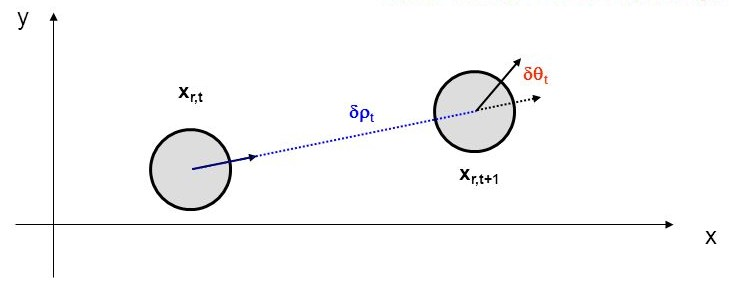
\includegraphics[width=8cm]{img/pose}
	\caption{Exemplo de poses que um robô pode assumir.}
	\label{img:pose}
\end{figure}

A segunda etapa do software de inteligência é responsável por verificar se uma nova pose de interesse $p_i$ foi definida para um robô $r_o$, caso sim, é executado um novo calculo da trajetória que ligará a pose atual $p_a$ do robô com a pose de interesse $p_i$. O calculo de trajetória é executado com auxílio da biblioteca OMPL (\textit{Open Motion Planning Library}) (Sucan et al, 2012)\cite{ompl} que implementa um apanhado de algoritmos de planejamento de trajetória, além de possibilitar otimizações quanto a suavidade do caminho gerado e o custo de movimento de uma pose atual para uma pose de interesse.

A terceira etapa do software de inteligência é feita em tempo de execução onde é utilizado a técnica campos potenciais (Goodrich, 2002)\cite{goodrich} para guiar os robôs de maneira reativa evitando colisões desenecessárias e seguindo suas trajetórias definidas na etapa anterior. Na figura \ref{img:myalgorithm} encontra-se a simulação de todas as etapas descritas.

\begin{figure}[thpb]
	\centering
	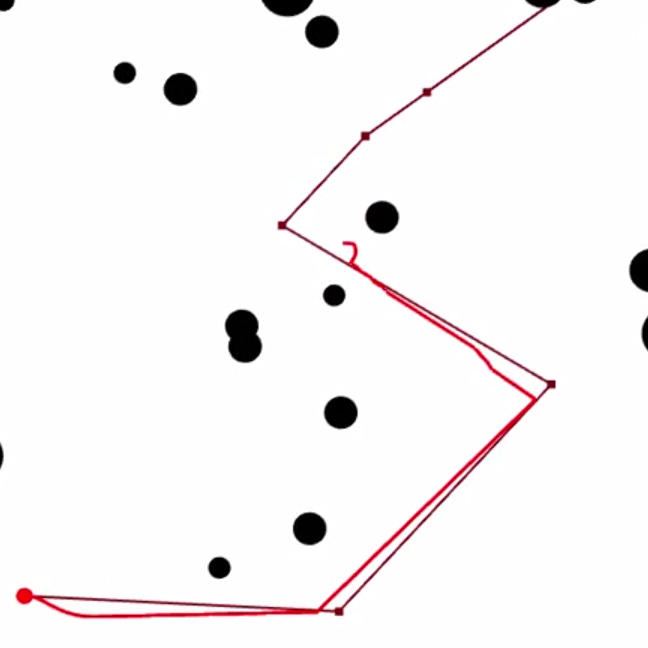
\includegraphics[width=8cm]{img/ex1}
	\caption{Simulação do algoritmo de inteligência.}
	\label{img:myalgorithm}
\end{figure}

\section{MECÂNICA E CONTROLE}
\subsection{Rodas omnidirecionais}
Para permitir movimento em todas as direções, rodas omnidirecionais são usadas nos robôs. Embora potência seja perdida, já que cada motor atua apenas com uma componente de sua velocidade, o ganho por ter liberdade de movimento em todas as direções é substancial, pois diminui o número de ações que o robô terá de executar para se movimentar, ou seja, tornando-o mais ágil. 

Para determinar as velocidades em cada motor sabendo as velocidades radial, tangencial e angular, uma matriz de transformação $D$ é utilizada. Multiplicando-a pela esquerda o vetor $v = [V_x$\hspace{0.25cm}$V_y$\hspace{0.25cm}$w_r]^T$ temos o vetor $m = [V_1$\hspace{0.25cm}$V_2$\hspace{0.25cm}$V_3$\hspace{0.25cm}$V_4]^T$, que diz as velocidades que cada motor deve gerar.

\begin{figure}[thpb]	
	\centering
	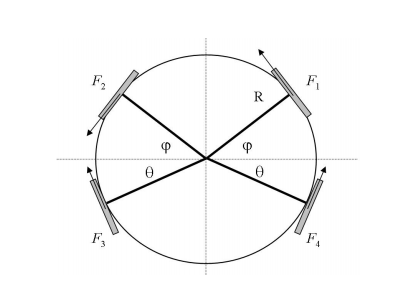
\includegraphics[width=8cm]{img/omni}
	\caption{robô visto de cima, com os respectivos ângulos para a matriz D. Fonte: \cite{omni}}
	\label{img:omni}
\end{figure}

Outra ferramenta interessante de usarmos essas rodas é verificar de forma simples se alguma roda está deslizando em uma camada acima do controle PID (Ogata, 2003)\cite{ogata-pid}. Para isso, calcula-se a pseudo-inversa de $D$, $D^+$, e verifica-se se ($I-D*D^+)*m$ = 0. Se for diferente de zero, quer dizer que há deslizamento. Para corrigir isto, pega-se a primeira linha da matriz $I-D*D^+$, gerando o vetor $u^T$. Então, o $m*$ corrigido será dado pela retirada da projeção de $m$ em $u$. Algebricamente, $m* = m - <m,u> u/<u,u>$. Desfeito o deslizamento, pode-se então proceder com o controle PID (Rojas, 2005)\cite{omni}.
 
\section{Eletrônica}
%Eletrônica
A fim de produzir uma geração nova de robôs, a quarta na história do time, o projeto eletrônico está sendo reformulada esse ano com base no projeto antigo, mas com pequenas alterações visando aumentar tornar o projeto mais organizado e otimizar o processo de produção. Com isso o desenho das placas está sendo refeito do zero utilizando uma ferramenta de projeto nova para o time o Altium Designer, sendo dada mais atenção ao dimensionamento das trilhas e escolha e posicionamento dos componentes.
A eletrônica dos robôs é baseada em uma arquitetura modular com foco em facilitar a rápida manutenção dos robôs em caso de falhas, manter baixo o custo de manutenção e tornar o projeto mais didático. O projeto eletrônica é dividida em 9 placas, uma placa mãe, 5 módulos de motor, um módulo de chute, um módulo de transmissão comercial o NRF24L01, um módulo de controle comercial (a stm32-discovery) e a placa mãe do robô.
Aproveitando as mudanças, o firmware do robô também está sendo reescrito para ser implementando o conceito de abstração de hardware e aumentando o caráter modular do projeto. Com esse objetivos em mente, o código está sendo mudado de C para C++, e foi dividido em classes que representam recursos físicos do microcontrolador e chips do robô. Também está se passando a utilizar um sistema operacional de modo a possibilitar o uso de threads.


\subsection{Módulo de controle}

\begin{figure}[thpb]	
	\centering
	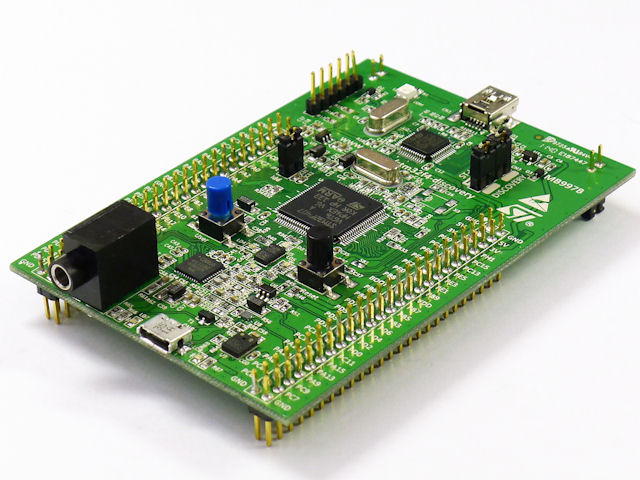
\includegraphics[width=8cm]{img/modulocontrole}
	\caption{Módulo de controle utilizado, placa STM32F4-Discovery. Fonte: \cite{omni}}
	\label{img:modulocontrole}
\end{figure}

O módulo de controle utilizado é uma placa comercial, a STM32F4-Discovery produzida pela STMicroelectronics e sua função é conter o microcontrolador STM32F407VG de arquitetura ARM32 Cortex M4, responsável por realizar as operações lógicas do robô servindo como cérebro do sistema eletrônico.
Está sendo implementado esse ano um sistema operacional no módulo de controle. Segundo (Maziero,2013)\cite{maziero}, os objetivos básicos de um sistema operacional podem ser sintetizados em abstração de hardware e gerência de recursos (quando dois ou mais aplicativos precisam dos mesmos recursos para poder executar e cabe ao sistema operacional definir políticas para gerenciar o uso dos recursos de hardware pelos aplicativos, e resolver eventuais disputas).
Um sistema operacional dá a ilusão de que há várias tarefas sendo executadas a cada momento fazendo com que o processador alterne rapidamente de tarefa e delegando a cada tarefa uma fração do tempo de uso de processador adequada para sua execução. Isso é feito pelo agendador de tarefas (scheduler). 
O scheduler em um RTOS (Real Time Operating System) é feito para ter um padrão de execução previsível (determinístico). Isso é particularmente interessante para sistemas embarcados, pois é necessário que o sistema responda a um evento dentro de um intervalo de tempo bem definido (chamado de deadline). Schedulers de tempo real tradicionais, tais como o usado no FreeRTOS, obtém determinismo permitindo ao usuário atribuir uma prioridade a cada linha de execução (thread). O scheduler usa a prioridade para saber qual a próxima thread executar.
Por fim, FreeRTOS é um RTOS gratuito, bastante popular, desenvolvido pela Real Time Engineers Ltd. para ser pequeno o bastante para ser usado em microcontroladores. FreeRTOS é distribuído sob a GPL (GNU Public License) com uma restrição adicional e uma exceção opcional que permite que o código do proprietário seja fechado, mantendo apenas o kernel código aberto.
Portanto, trata-se de um sistema operacional que permitirá a execução “simultânea” de tarefas de controle dos motores e comunicação do robô com a inteligência, atribuindo a cada tarefa uma fração de tempo determinada, sem aumentar muito o consumo de memória e usando um software gratuito e amplamente difundido.

\subsection{Módulo do motor}

\begin{figure}[thpb]	
	\centering
	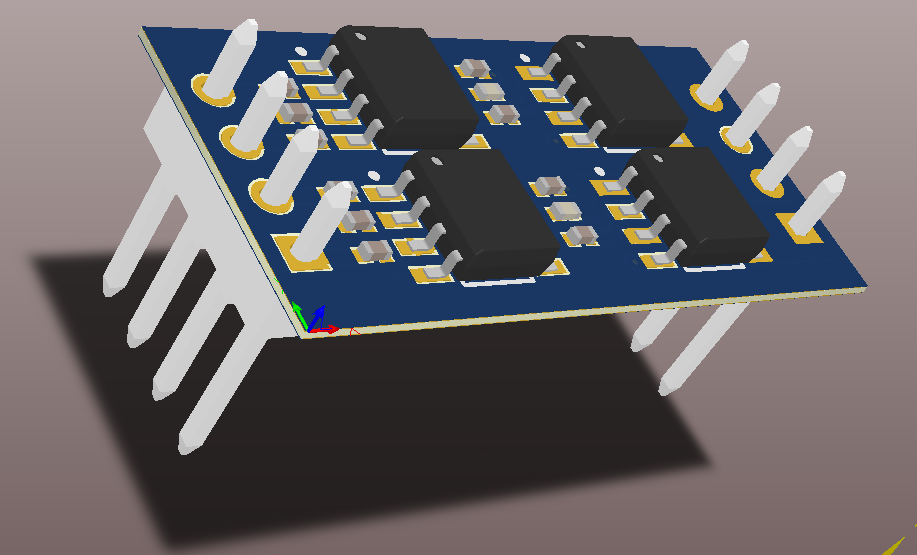
\includegraphics[width=8cm]{img/modulomotor}
	\caption{Módulo do motor.}
	\label{img:modulomotor}
\end{figure}

Os módulos de motor são responsáveis por fazer o controle dos quatro motores responsáveis pelo movimento do robô e do motor responsável pela atuação do driblador. E consiste em uma ponte H capaz de controlar a velocidade de um motor de corrente contínua em duas direções. 
A placa é controlado pelo microcontrolador através da classe motor que utiliza a classe encoder para determinar a velocidade instantanea do motor, com essa velocidade utiliza um algorítmo de controle PID para calcular a resposta que deve ser transmitida a placa, e envia essa resposta utilizando as classes degrau unitário e PWM (pulse width modulation).
O circuito de ponte H permite que o microcontrolador controle o sentido de rotação dos motores e a potência transmitida a eles, através do chaveamento dos transistores internos da ponte e amplificando o sinal enviado pelo microcontrolador.
O desenho dessa placa foi reformulado esse ano, as trilhas foram trocadas por planos nos caminhos de potência e foram adicionados um par de capacitores de desaclopamento na entrada dos drivers dos transistores.
Está sendo implementado ainda esse ano um algoritmo de controle para evitar o deslizamento rodas omnidirecionais usadas no robô, baseado no artigo [1].
Para determinar as velocidades em cada motor sabendo as velocidades radial, tangencial e angular, uma matriz de transformação D é utilizada. Multiplicando-a pela esquerda o vetor $v = [V_x V_y wr]^T$ temos o vetor $m = [V_1 V_2 V_3 V_4]^T$, que diz as velocidades que cada motor deve gerar.
\begin{equation}
    D=\left[\begin{array}-\sin\phi   \quad \cos\phi     \quad 1\\
                         -\sin\phi   \quad -\cos\phi    \quad 1\\
                          \sin\theta \quad -\cos\theta  \quad 1\\
                          \sin\theta \quad \cos\theta   \quad 1
    \end{array}\right]
\end{equation}
%D =[-sin(phi) cos(phi) 1;
%-sin(phi) -cos(phi) 1;
%Sin(theta) -cos(theta) 1;
%Sin(theta) cos(theta) 1]

Figura 1: robô visto de cima, com os respectivos ângulos para a matriz D. Fonte: [1]
Outra ferramenta interessante de usarmos essas rodas é verificar de forma simples se alguma roda está deslizando em uma camada acima do controle PID. Para isso, calcula-se a pseudo-inversa de $D$, $D^+$, e verifica-se se $(I-D*D^+)*m = 0$. Se for diferente de zero, quer dizer que há deslizamento. Para corrigir isto, pega-se a primeira linha da matriz $I-D*D^+$, gerando o vetor $u^T$. Então, o $m^*$ corrigido será dado pela retirada da projeção de m em u. Algebricamente, $m^* = m -  u\displaystyle\frac{<m,u>}{<u,u>}$. Desfeito o deslizamento, pode-se então proceder com o controle PID. [1]

\subsection{Placa mãe}

A placa mãe é responsável por fazer a ligação entre os atores do robô, transmitindo potência da bateria para os módulos de motor e de chute, fazendo a ligação entre esses módulos e os respectivos atuadores, fornecendo tensão aos circuitos lógicos e fazendo a ligação entre o módulo de controle e os sensores do robô -, no caso um sensor de quadratura em cada motor e o sensor ótico do chute que verifica a posse da bola. 
Para que as ligações feitas pela placa sejam feito de modo estável e seguro a placa mãe contém um fusível, um capacitor de tanque, um capacitor de desacoplamento, e um sensor de corrente, o chip INA220, na entrada de cada módulo de motor e na entrada do módulo de chute, além de um circuito de divisão de tensão para que o módulo de controle seja capaz de controlar o nível de tensão da bateria.
O controle dessa placa é feito através da classe da INA220 no firmware que faz a comunicação com os sensores de corrente na placa e a classe bateria que controla o nível da bateria sendo usada pelo robô. Essas classes permitem o controle dos circuitos de segurança do robô de maneira que o firmware possa lidar com comportamento anômalos.
O desenho dessa placa foi reformulado esse ano, as trilhas nos caminhos de potência foram trocados por planos, os antigos fusíveis simples foram trocados por fusíveis restáveis para evitar a troca em cada caso de comportamento anômalo. E os capacitores de tanque thrue holes foram trocados por capacitores smd visando automatizar o processo de montagem utilizando uma pick and place automática.
Os sensores de corrente também foram trocados por sua versão mais moderna e foi corrigido um erro em sua implementação no esquemático. Outra pequena mudança foi a troca do conector do módulo de transmissão para ser compatível com o novo módulo de transmissão adotado pelo time.

\subsection{Módulo de chute}

O mecanismo de chute do robô foi elaborado utilizando dois solenoides como atuadores, um responsável pelo chute para frente e outro responsável pelo chute alto. E a placa é responsável por produzir a alta tensão necessária para ativar os dois solenoides, e transmitir a energia acumulada para acionar os atuadores.
A placa funciona através de um circuito de conversão DC-DC controlado pelo circuito integrado MC34063 que converte os 7,8V DC da bateria em uma saida de 180V DC ligada a dois capacitores eletrolíticos de 2200 UF e 200V. Além desse circuito existe ainda um circuito para chavear a tensão dos capacitores nos solenoides, o que é feito utilizando um TC4427 driver de mosfet e dois mosfets de potência IRFP4868PBF. 
O controle desse módulo é feito através da classe chute que utiliza a classe degrau unitário para limitar a energia transmitida a bola alterando a duração do intervalo de tempo que os mosfets ficarão ativados.

\subsection{Módulo de transmissão}

\begin{figure}[thpb]	
	\centering
	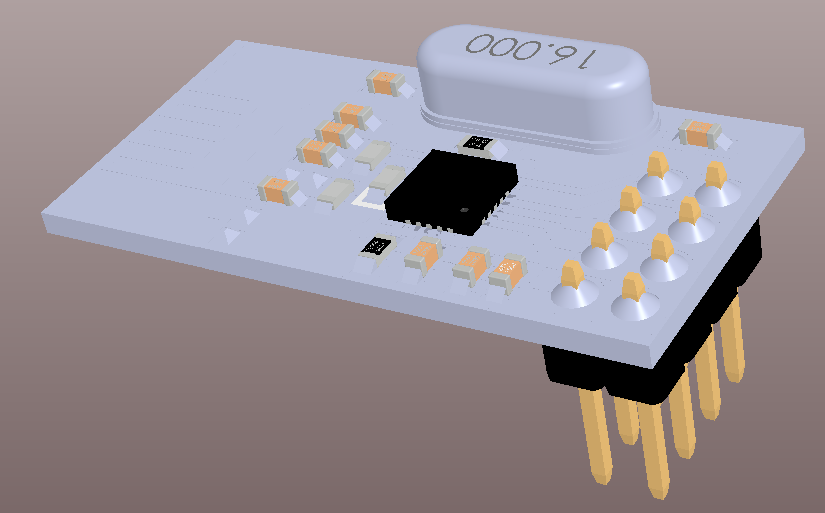
\includegraphics[width=8cm]{img/modulotransmissao}
	\caption{Módulo de transmissão. Placa comercial baseada no chip NRF24L01}
	\label{img:modulotransmissao}
\end{figure}

	Esse módulo é responsável pela comunicação entre a inteligência e o módulo de controle do robô. Consiste em uma placa comercial contendo o chip NRF24L01 e os periféricos necessários para o seu uso.
O módulo é ligado ao módulo de controle do robô através da placa mãe e se comunica com este utilizando o protocolo SPI. Para fazer a comunicação com a inteligência, o módulo se comunica com outro igual ligado ao computador onde a inteligência está sendo executada utilizando uma frequência na faixa de 2,4 GHz.
Para a comunicação entre dois módulos, o chip utiliza um protocolo próprio chamado Enhanced ShockBurst™, uma camada de vínculo de dados (camada de protocolo que lida com a entrada e saída de sequências de bits no meio físico, escondendo das camadas superiores o hardware subjacente e lidando com os pacotes perdidos e os pacotes duplicados) que permite envio de pacotes de confirmação sem a necessidade de receptor e transmissor inverterem seus modos de funcionamento (funcionalidade chamada Auto Acknowledgement). Isso permite ganhar tempo no envio das informações que a inteligência precisa. 
O Enhanced ShockBurst™ também permite o uso de até 6 pipes para o recebimento de mensagens e o envio de pacotes com tamanho variável. Outras funções desempenhadas são a montagem e desmontagem de pacotes, bem como a validação dos pacotes recebidos, sendo necessário apenas configurar alguns registradores, simplificando o código da transmissão.
Embora o rádio ofereça a opção de usar CRC para verificar erros nos pacotes, isso não foi usado, pois tornaria a recepção mais lenta (devido à verificação que seria feita) e durante os testes as mensagens nunca chegavam corrompidas.


\section{Mecânica}

Design Mecânico

2. Design Mecânico
Esse robô foi e esta sendo desenhado utilizando-se de software de CAD(Computer Aided
Design) e CAM(Computer Aided Manufacturing). Vários melhoramentos e testes estão sendo
feitos para melhorar o projeto herdado dos antigos membros da equipe visando
principalmente em:
a) Deixar o projeto mais simples, se atentando a facilitar a produção das peças e
retirando as desnecessárias;
b) Eficiente, ou seja, que tenhamos uma melhorar na precisão do controle e peças
mais resistentes.
A maioria de nossas peças são feitas através de maquinas que utilizam o método
CNC(Computer Numeric control) e feitas de alumínio 70-75 apresentando uma alta resistência
mecânica e são boas de serem usinadas, sendo o restante em PLA material que foi utilizado
pela impressora 3D e tentaremos usar plástico injetado em alta pressão.
\begin{figure}[thpb]	
	\centering
	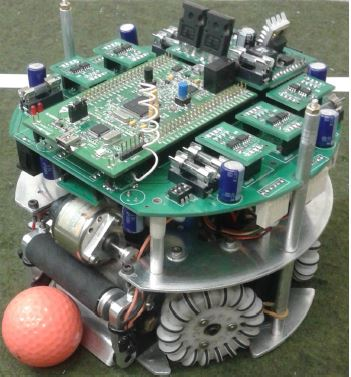
\includegraphics[width=4.5cm]{img/mec1}
	\caption{Módulo do motor.}
	\label{img:modulomotor}
\end{figure}
\begin{figure}[thpb]	
	\centering
	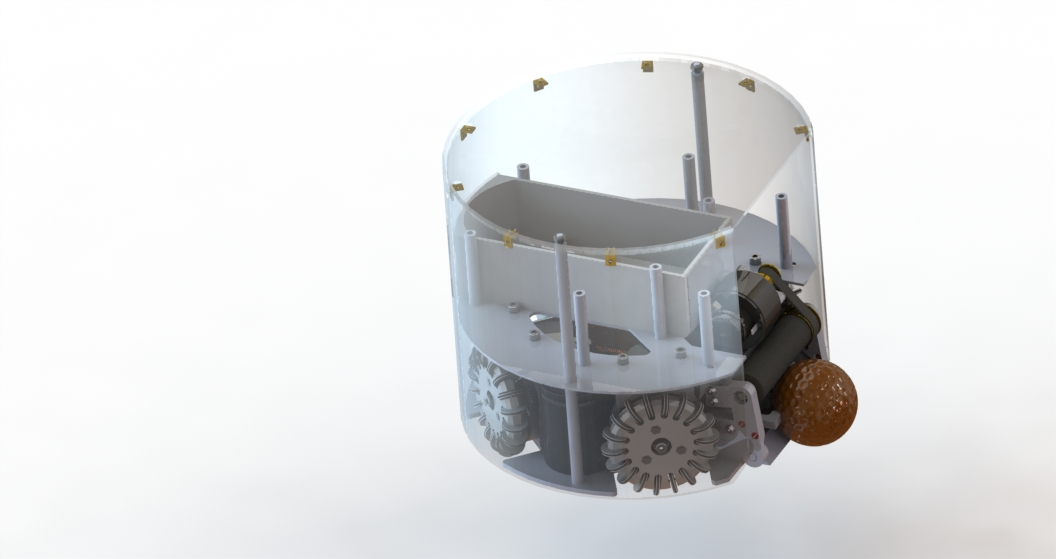
\includegraphics[width=4.5cm]{img/mec2}
	\caption{Módulo do motor.}
	\label{img:modulomotor}
\end{figure}
2.1 Métodos de produção
2.1.1 Usando corte com jato d’água (jet-cutting) produzimos o chassi e a base superior
que divide a eletrônica e a bateria do resto do Robô, para isso usamos placas de alumínio de
3mm e 2.5 mm respectivamente.
\begin{figure}[thpb]	
	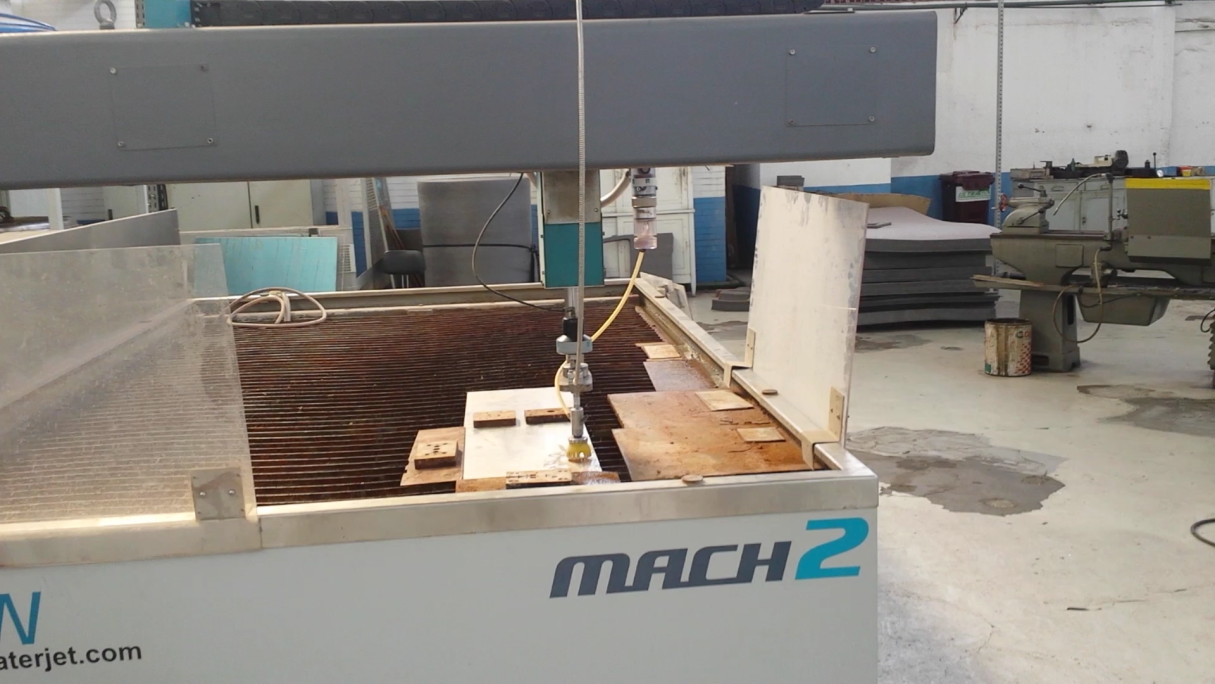
\includegraphics[width=2.5cm]{img/mec3}
	\caption{Módulo do motor.}
	\label{img:modulomotor}
\end{figure}
\begin{figure}[thpb]	
	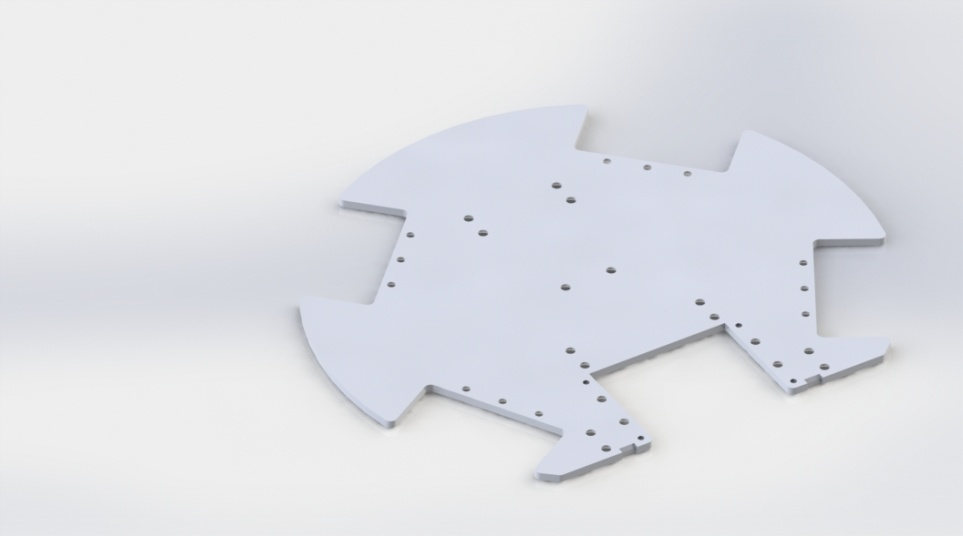
\includegraphics[width=2.5cm]{img/mec4}
	\caption{Módulo do motor.}
	\label{img:modulomotor}
\end{figure}
\begin{figure}[thpb]	
	\centering
	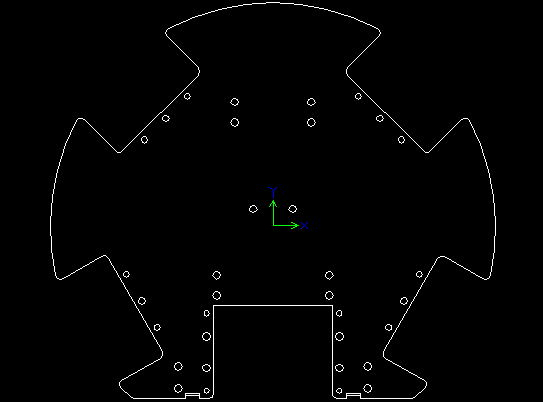
\includegraphics[width=4.5cm]{img/mec5}
	\caption{Módulo do motor.}
	\label{img:modulomotor}
\end{figure}
2.1.2 Usando a fresadora CNC, produzimos a maioria de nossas peças após a modelagem CAD
das peças tínhamos que fazer o CAM para gerar o código máquina. Algumas peças foram
bastante desafiadoras tendo em vista o tamanho reduzido e a complexidade de algumas
peças. Esses dois fatores afetaram principalmente a tirada de referências da peça com o
apalpador da máquina, afim de pressetar a origem, e como prenderíamos essa peça na morsa
de maneira segura, principalmente nas ultimas fases da produção da peça.
\begin{figure}[thpb]	
	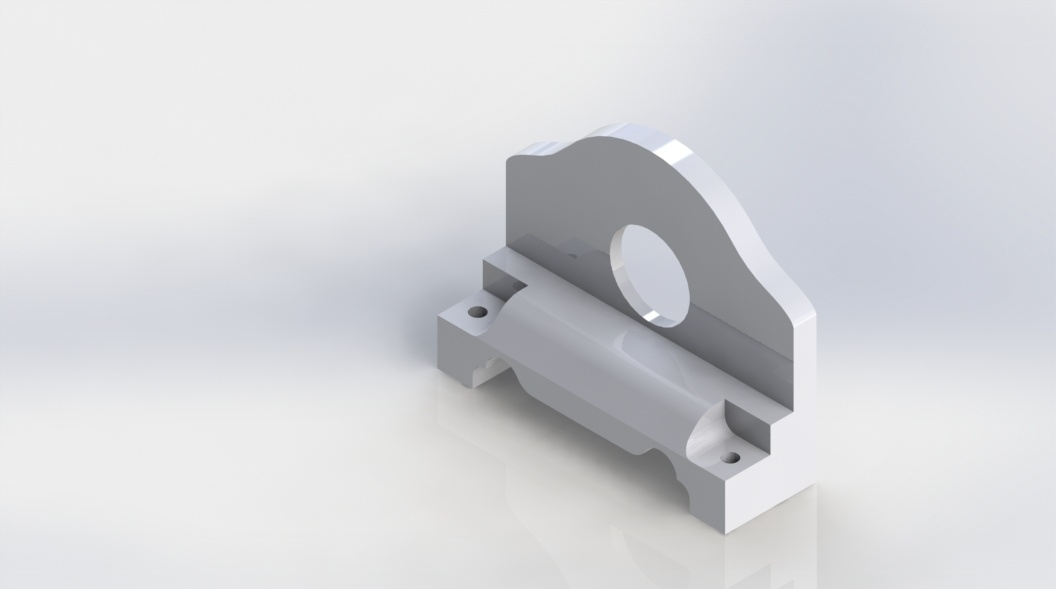
\includegraphics[width=2.5cm]{img/mec6}
	\caption{Módulo do motor.}
	\label{img:modulomotor}
\end{figure}
\begin{figure}[thpb]	
	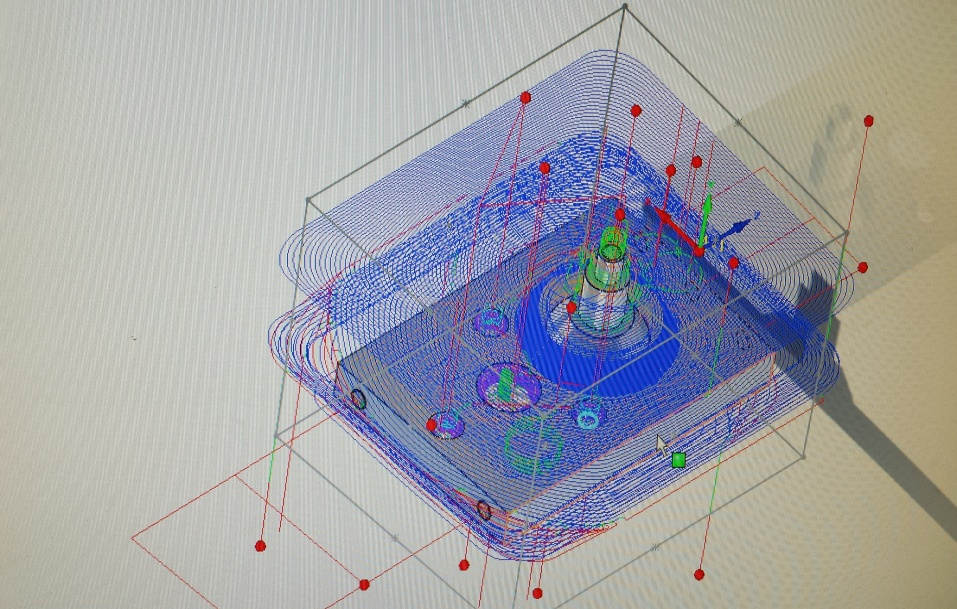
\includegraphics[width=2.5cm]{img/mec7}
	\caption{Módulo do motor.}
	\label{img:modulomotor}
\end{figure}
2.2.3 Por fim foi utilizadas ferramentas como impressora 3D, tornos, jateamento, pneumática
seja para produção ou acabamento de peças.
\begin{figure}[thpb]	
	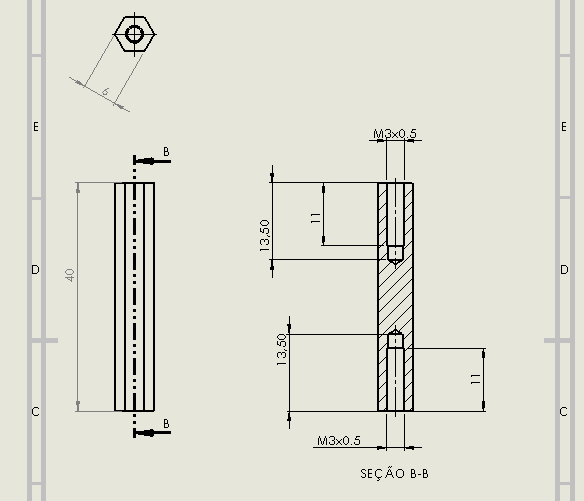
\includegraphics[width=2.5cm]{img/mec8}
	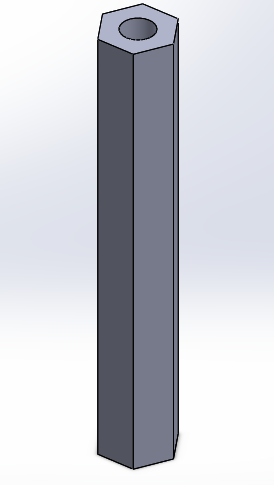
\includegraphics[width=2.5cm]{img/mec9}
	\caption{Módulo do motor.}
	\label{img:modulomotor}
\end{figure}
\begin{figure}[thpb]	
	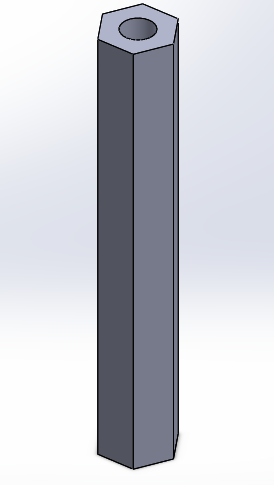
\includegraphics[width=2.5cm]{img/mec9}
	\caption{Módulo do motor.}
	\label{img:modulomotor}
\end{figure}
2.3 Dimensões
Em conformidade com as regras de SSL, a altura do robô é de 149 mm e a projeção máxima do
robô no solo é de 180 mm. A altura do driblador é ajustável, de modo que somos capazes de
encontrar o ponto ideal para o melhor controle de bola. Utilizando software de CAD, fomos
capazes de medir a porcentagem de área da bola que estava coberta pelo robô. Obtendo uma
porcentagem máxima de cobertura bola de 19,8\%, de acordo com o 20/80 regra da liga.
\begin{figure}[thpb]	
	\centering
	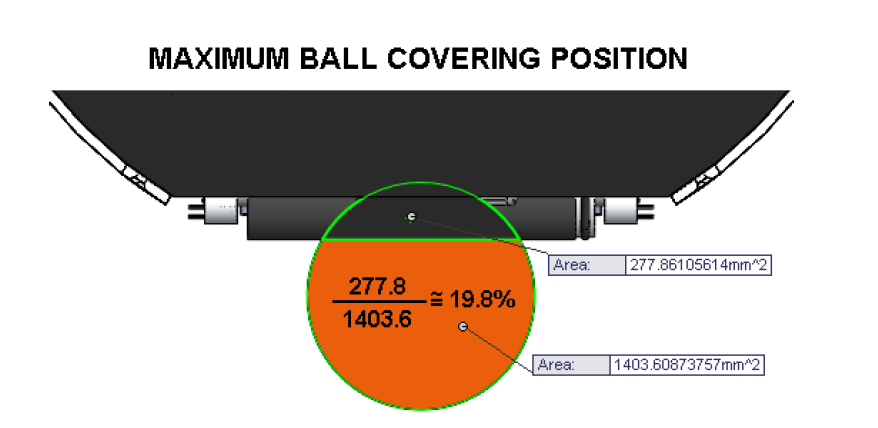
\includegraphics[width=8cm]{img/mec10}
	\caption{Módulo do motor.}
	\label{img:modulomotor}
\end{figure}
2.4 Sistema de Transmissão
Um sistema de engrenagens internas foi feito para transferir a potência dos motores de para
as rodas. Esse sistema tem várias vantagens quando comparado com o método tradicional, 
como evitar a entrada de detritos os motores, cria uma cavidade para aplicar graxa para a
lubrificação de engrenagens e um tamanho total menor.
No entanto, existem algumas dificuldades na fabricação dessa peça, principalmente devido ao
pequeno tamanho dos dentes, necessários para engrenar com a engrenagem do motor padrão
(o motor utilizado é o Hsiang Neng DC escovado motor do tipo HN-GH35GMB). No este motor
a distância entre dois dentes consecutivos é inferior a 1 mm, ficando difícil de usinar a
engrenagem interna para essa peça.
Antigamente foi utilizado impressora 3D para imprimir em plástico ABS a peça, porém as
peças não apresentaram bons rendimentos, quebrando a peça e os dentes facilmente, fora
que muitas não apresentavam um movimento suave, travando se a força imprimida para sua
rotação não fosse significante, o que dificultava o controle do robô, assim tentaremos usar o
método de eletroerosão para contornar problema do pequeno tamanhos dos dentes. Assim
poderíamos usinar um molde, que serviria para produzir as peças através de injeção.
Se essa opção não funcionar, podemos fazer o molde em impressora 3D, criando uma
proteção para a parte que o plástico entra ou encomendar um molde de uma empresa
especializada.
2.5 Chute
O chute rasteiro é formado por um conjunto de placa de chute, pistão, suporte dianteiro do
solenoide, suporte traseiro do solenoide e solenoide. Ele é ativado através de dois capacitores
que energizam o solenoide fazendo o pistão, que está aclopado com a placa, ser impulsionado
para frente.
Chute alto é formado por placa de chute, suporte único do solenoide, pistão,solenoide,
suporte para retenção do pistão.
Em ambos casos estamos usando ligas para trazer de volta os pistões, por serem baratas e
eficientes no processo, porem no caso do chute rasteiro esta sendo estudado mudar para uma
mola cônica, ou ambos casos fazer uma volta invertendo a corrente do solenoide, mas essa
opção consumiria energia o que não é interessante
\begin{figure}[thpb]	
	\centering
	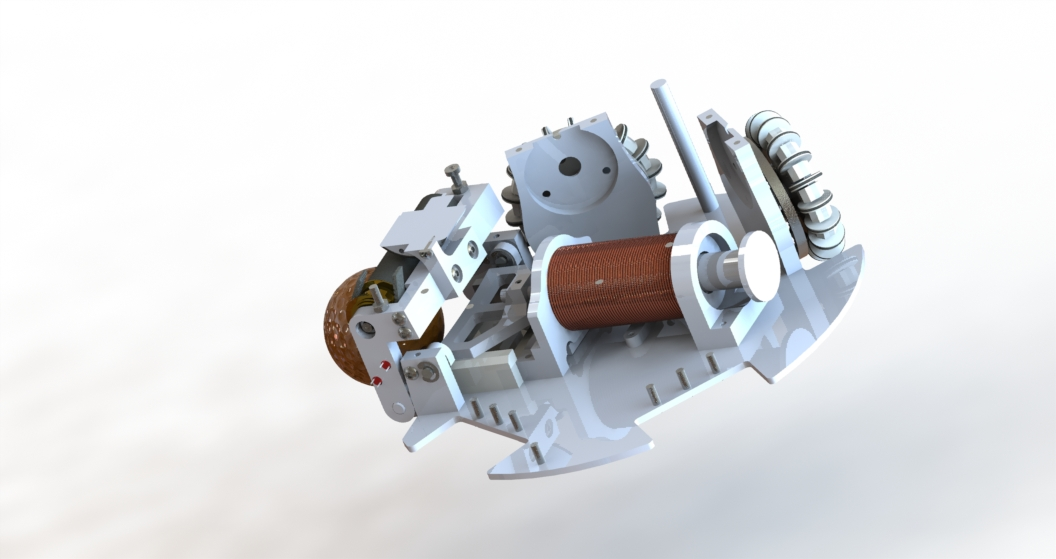
\includegraphics[width=8cm]{img/mec11}
	\caption{Módulo do motor.}
	\label{img:modulomotor}
\end{figure}

\section{CONCLUSÃO}

\bibliographystyle{unsrt}
\footnotesize\bibliography{ref}		



\end{document}
